% Chapter Template

\chapter{Results} % Main chapter title

\label{Results} % Change X to a consecutive number; for referencing this chapter elsewhere, use \ref{ChapterX}

%----------------------------------------------------------------------------------------
%	SECTION 1
%----------------------------------------------------------------------------------------
\section{Machine learning}

The convolutional neural network (CNN) was initially trained on the labelled dataset provided by \cite{Hill2018} and this proved highly successful, with 95\% accuracy acheived when presented with test data from the same dataset. I then fed data from the Osa Peninsula through this model and it returned 6912 'gunshots'. I manually validated these 'gunshots' through auditory inspection and determined that 252 were authentic gunshots, giving a model precision of 3.65\%. I then re-trained the CNN on the new, manually-labelled dataset from the Osa Peninsula, and tested it by feeding through data from the Osa Peninsula that had not been used to train it. This model returned approximately five times as many 'gunshots'. I then assembled a combined training dataset, consisting of the data provided by \cite{Hill2018} and the new labelled data from the Osa Peninsula. The model trained on this dataset returned approximately 15 times more 'gunshots' then the original Belize model. Finally, I assembled a new training dataset consisting only of labelled data from the Osa Peninsula, but this time the spectra labelled as negatives were false positives that I had previously identified. Upon testing, this model returned about 4\% fewer 'gunshots' than the original Belize model. The number of 'gunshots' found by each variant of the model is highlighted in Figure ~\ref{fig:model_comparison}.


\section{Spatio-temporal analysis}

Using only the authenticated gunshots from the Belize model, I undertook further analysis to explore the temporal patterns of hunting (Figure ~\ref{fig:weekday_plot}). Firstly, a chi-square test of goodness-of-fit was performed to determine whether gunshot frequency was independent of the day of the week. Gunshot frequency was equally distributed across the weekdays, $X^2$ (25, $N$ = 252) = 42, $p$ = 0.227. I then conducted a negative binomial regression on the effect of day-of-the-week on gunshot frequency as this has been shown to be an appropriate method for modelling overdispersed count data \citep{Zeilis2008}. This model showed that there is evidence that the days 'Monday' ($e^{estimate}$ = 2.50, z = 2.62, $p$ < 0.009), 'Wednesday' ($e^{estimate}$ = 3.53, z = 2.85, $p$ < 0.004), 'Friday' ($e^{estimate}$ = 3.47, z = 2.81, $p$ < 0.005), and 'Saturday' ($e^{estimate}$ = 2.67, z = 2.81, $p$ < 0.029) are significant predictors of gunshot frequency.  \\

\noindent I then conducted similar analysis on the time of day gunshots occured (Figure ~\ref{fig:timeday_plot}). Gunshots were assigned to either 'morning', 'afternoon', or 'night', mirroring the three periods of the day that the audio sensors were set to record. A chi-square test of goodness-of-fit was performed to determine whether gunshot frequency was independent of time of day. Gunshot frequency was equally distributed across the three periods of the day, $X^2$ (4, $N$ = 252) = 6, $p$ = 0.199. As before, I carried out negative binomial regression on the effect of time of day on gunshot frequency. This model showed that there is evidence that 'Morning' is a significant predictor of gunshot frequency ($e^{estimate}$ = 3.07, z = 7.07, $p$ < 0.0001). 'Night' was also shown to be a significant predictor of gunshot frequency ($e^{estimate}$ = 0.26, z = -4.75, $p$ < 0.0001). \\

\noindent Gunshot frequency between the six study areas was also compared (Figure ~\ref{fig:area_plot}). A chi-square test of goodness-of-fit was performed to determine whether gunshot frequency was independent of area. Gunshot frequency was equally distributed across the six areas, $X^2$ (25, $N$ = 252) = 30, $p$ = 0.224.

\begin{figure}\centering
\subfloat[]{\label{}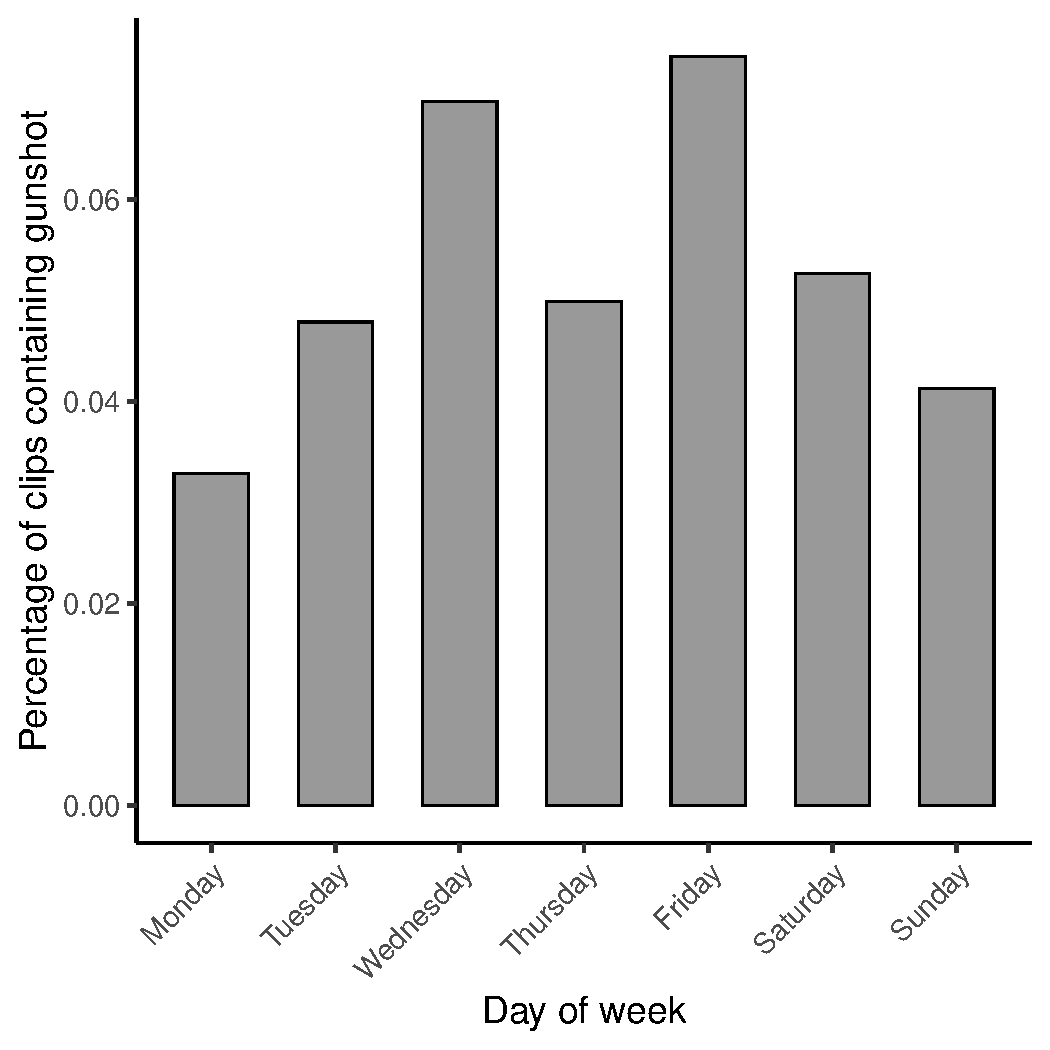
\includegraphics[width=.48\linewidth]{weekday_plot}}\hfill
\subfloat[]{\label{}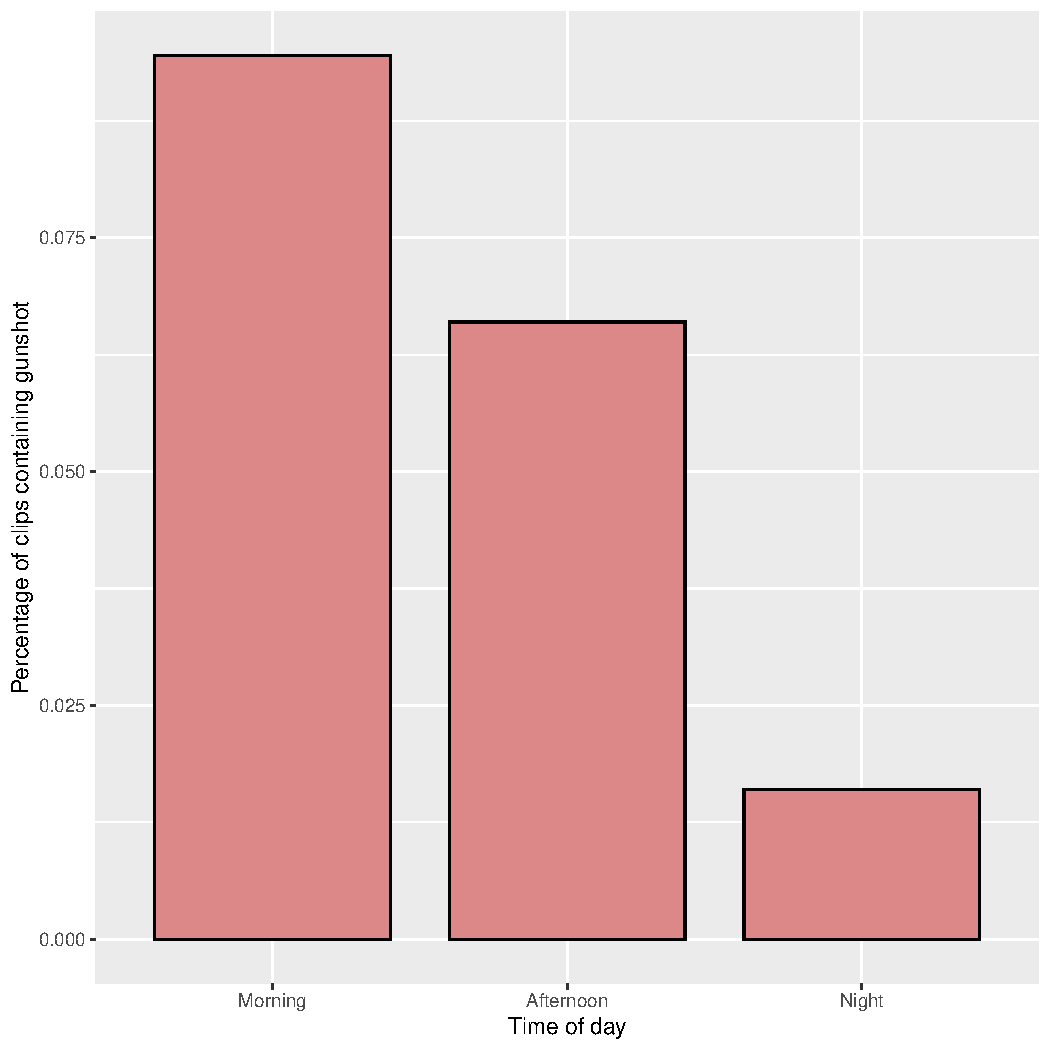
\includegraphics[width=.48\linewidth]{timeday_plot}}\par
\subfloat[]{\label{}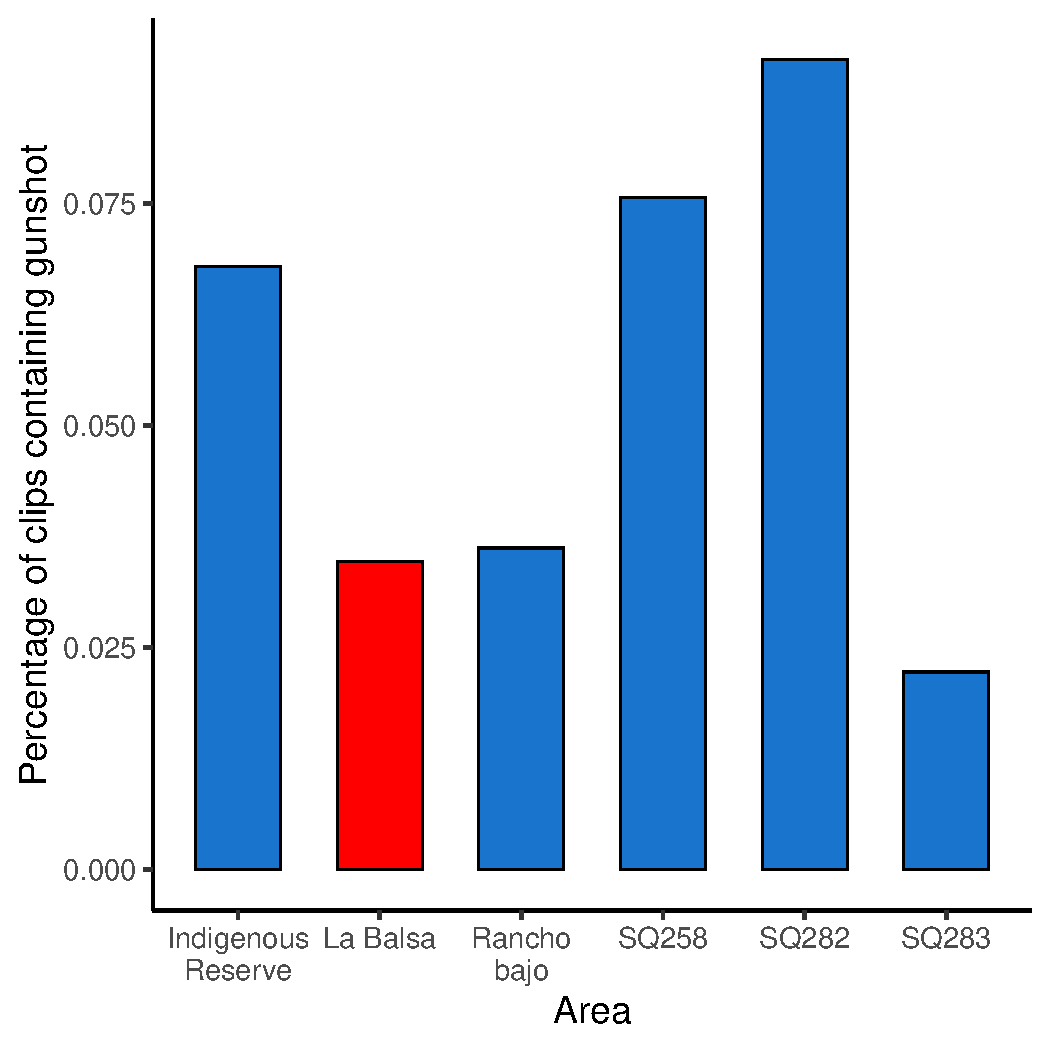
\includegraphics[width=.48\linewidth]{area_plot}}
\caption{}
\label{fig}
\end{figure}




\begin{figure}
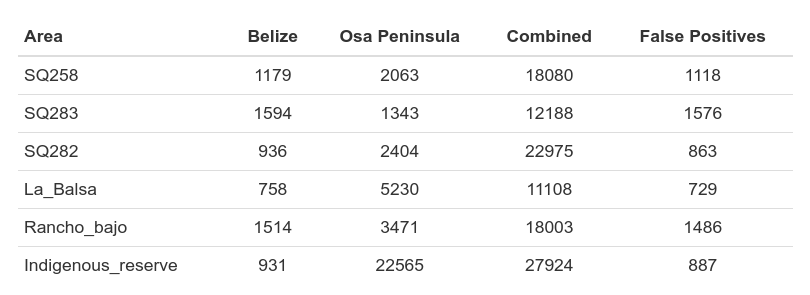
\includegraphics[width=1.2\textwidth,center]{Figures/model_comparison}\caption[Model comparison]{Number of returned 'gunshots' from each version of the convoluted neural network (CNN). The 'Belize' model was trained only on data provided by \cite{Hill2018}, 'Osa Peninsula' was trained on data collected by Jenna Lawson \citep{Lawson2019}, 'Combined' was trained on a combination of the previous two datasets, and 'False Positives' was trained on Jenna's data but all negatives provided were previously identified false positives.}\label{fig:model_comparison}
\end{figure}



\begin{table}[!h]
\centering
\begingroup\footnotesize
\begin{tabular}{rrrrrrr}
  \hline
 & Estimate & Exponential & S.E. & z-value & 95\% C.I. & p-value \\
  \hline
Monday & 0.92 & 2.50 & 0.35 & 2.62 & from 1.24 to 4.95 & 0.009 \\
  Tuesday & 0.73 & 2.07 & 0.46 & 1.59 & from 0.85 to 5.14 & 0.11 \\
  Wednesday & 1.26 & 3.53 & 0.44 & 2.85 & from 1.50 to 8.56 & 0.004 \\
  Thursday & 0.79 & 2.20 & 0.46 & 1.73 & from 0.91 to 5.45 & 0.083 \\
  Friday & 1.24 & 3.47 & 0.44 & 2.81 & from 1.47 to 8.41 & 0.005 \\
  Saturday & 0.98 & 2.67 & 0.45 & 2.18 & from 1.11 to 6.54 & 0.029 \\
  Sunday & 0.38 & 1.47 & 0.47 & 0.81 & from 0.58 to 3.74 & 0.42 \\
   \hline
\end{tabular}
\endgroup
\caption{NegBin model. Estimated dispersion: 3.02 ($se=1.09$).}
\label{tab:glm.nb}
\end{table}


\begin{table}[!h]
\centering
\begingroup\footnotesize
\begin{tabular}{rrrrrrr}
  \hline
 & Estimate & exp.estimate & S.E. & z-value & 95\% C.I. & p-value \\
  \hline
Morning & 1.12 & 3.07 & 0.16 & 7.07 & from 2.26 to 4.22 & $<$ 0.0001 \\
  Afternoon & -0.22 & 0.80 & 0.24 & -0.95 & from 0.50 to 1.27 & 0.34 \\
  Night & -1.34 & 0.26 & 0.28 & -4.75 & from 0.15 to 0.45 & $<$ 0.0001 \\
   \hline
\end{tabular}
\endgroup
\caption{NegBin model. Estimated dispersion: 1.41 ($se=0.35$).}
\label{tab:glm.nb_time}
\end{table}
